%%% Local Variables:
%%% mode: latex
%%% TeX-master: t
%%% End:

% !Mode:: "TeX:UTF-8"

\chapter{MPSoC结构级热分析的实验数据与分析}
\label{cha:SSTAexperiments}

\section{实验平台与测例说明}
为了检验本文所提出的模块级、核级、改良核级3种热分析方法的精度与效率,选择热分析软件HotSpot-5.02作为验证基准, 构建了3个测例进行温度-功耗数据对比分析。工作的硬件平台为配有Intel Core i7,8G RAM,运行Windows7和Ubuntu 12.04 LTS双系统的PC机。

测例1. 采用文献\onlinecite{LrnAutoRegMdlFstTransThemAlysCp}策略,首先构建了基于Alpha21264核心的4核处理器。 对于这4个物理核,每个核有两块独享缓存L2\_Right、L2\_Left,4个核共享最后一级缓存L3。 考虑处理单元的片上散热问题,将处理核心放置于芯片边缘。将共享缓存区置于芯片中心, 这样将有利于通过功率较低的共享缓存, 隔断功率较大的多个核相互之间的热交换影响。每个核的独享缓存处于核的周围。 根据表2中所示参数,重复地随机产生功耗分布,考虑电热耦合效应,分别采用BloTAM、CorTAM和BiCorTAM方法, 分别对其温度分布进行计算,并与HotSpot结果进行对比。
测例2. 对于采用Intel Sandy Bridge-E架构的8核高端CPU芯片\onlinecite{INTELi7} ,其核心面积为435平方毫米,长度和宽度分别为20.9毫米、20.8毫米,基本呈正方形。 本文按照其布局原则模拟生成了一种较为简略的芯片布局结构。根据表2所示的参数设置方案, 重复地随机产生确定的功耗分布, 针对每种功率分布;考虑电热耦合效应,分别采用本文的3种热分析方法、来获得每个功率分布的温度稳定分布, 以分析它们的求解精度。
测例3. 基于测例1采用的Alpha21264核心,本文构建一个16核的虚拟芯片进行温敏布图规划,并对布图方案进行热分析, 以测试本文方法的运行效率。

\section{方法分析精度的实验数据与分析}
本文先按照表2中设定的参数、产生100个输入向量,然后采用HotSpot、BloTAM、BioCorTAM、CorTAM这4种方法 来测试各个核与功能模块的温度与静态功耗,其中一个核的静态功耗值等于所属模块的静态功耗值之和, 这个核的局部热点温度是它的Core\_x模块温度。本文采用HotSpot的测值作为基准、来求解其余3种方法的相对误差。 由于芯片的工作温度均是相对环境温度$T_{ambient}$,本文使用式~\ref{equ:chap5:et}来计算温度误差$E_T$:
\begin{equation}
\label{equ:chap5:et}
E_T = |\frac{T-T_{HOTSPOT}}{T_{HOTSPOT}-T_{ambient}}|
\end{equation}
其中$T_{HOTSPOT}$是HotSpot的测值,$T$是本文方法的温度计算值。同时,本文采用下式来计算静态功耗误差$E_{Plk}$:
\begin{equation}
\label{equ:chap5:eplk}
E_{Plk} = |\frac{Plk-Plk_{HOTSPOT}}{Plk_{HOTSPOT}}|
\end{equation}
式~\ref{equ:chap5:eplk}中$Plk_{HOTSPOT}$是HotSpot的静态功耗测值,$Plk$是本文方法的静态功耗计算值。
本文3种方法的温度误差如表3所示。BloTAM的精度最高,平均误差小于1.6\%,最大误差小于5\%;BiCorTAM的精度次之, 平均误差小于4.2\%,最大误差小于15\%;CorTAM的精度最低,平均误差达到33\%,最大误差达到45\%。 因此,BloTAM和BiCorTAM 2种方法均可以提供满意的计算精度。
本文3种方法的静态功耗误差如表4所示。BloTAM的精度最高,最大误差小于0.5\%;BiCorTAM的精度次之, 平均误差小于1.2\%, 最大误差小于3.7\%;CorTAM的精度最低,平均误差达到25\%,最大误差达到35\%。因此,BloTAM和BiCorTAM 2种方法均可以提供满意的计算精度。

为了考察本文方法的误差来源,用图~\ref{fig:ex1-plk-error}和图~\ref{fig:ex1-temp-error}给出了对测例1中的 各个模块, 本文3种方法所产生的静态功耗与温度相对误差。以下内容是本文关于本文3种方法的误差分析:
(1)BloTAM方法的误差分析。由于BloTAM是基于HotSpot软件模拟出来的模块温度结果进行自下而上的建模, 所以该方法具有与HotSpot软件近似的精度。如图~\ref{fig:ex1-plk-error}所示,各模块的静态功耗误差小于0.3\%; 如图~\ref{fig:ex1-temp-error}所示,各模块的温度误差小于4\%。
(2) CorTAM方法的误差分析。在测例1一个核内,高功耗(高发热量)的Core\_x模块是高温模块, 其总功耗中静态功耗所占的比例高, 而其他3个模块L2\_x、L2\_Left\_x、 L2\_Right\_x是低功耗的低温模块,其静态功耗所占的比例也低。如图~\ref{fig:ex1-plk-error}所示, 由于产生局部热点的Core\_x模块温度明显高于其他核内模块, CorTAM假设核中所有模块的温度均为核的局部热点温度,与事实有着较大的出入, 导致其所计算出来的低温模块静态功耗明显偏大, 产生了11\%-15\%的较大误差。事实上,高温模块的温度就是核内的局部热点温度, 所以CorTAM所计算出来的高温模块静态功耗较为精确, 其相对误差小于2\%。由于低温模块的静态功耗计算误差明显偏大, 以核内所有模块功耗总和来计算核的局部热点温度就会产生较大的误差; 如图~\ref{fig:ex1-temp-error}所示,其所产生的温度误差处于6\%-8\%之间,明显大于其他2种方法。
(3) BiCorTAM方法的误差分析。该方法正视核内模块温度之间的明显差别,仅将核外模块作为一个影响整体进行考虑, 但由于仅将热点之间的相关热阻作为核间影响的系数,所以该方法对于热点温度可以提供较高的精度, 但其对于核内低温模块的温度计算精度则较差。如图~\ref{fig:ex1-plk-error}所示,各模块的静态功耗误差小于0.7\%; 如图~\ref{fig:ex1-temp-error}所示, 产生热点的高温模块的温度误差小于2.2\%,但低温模块的温度误差则达到了5\%-11\%。

\begin{figure}[H]
  \centering
  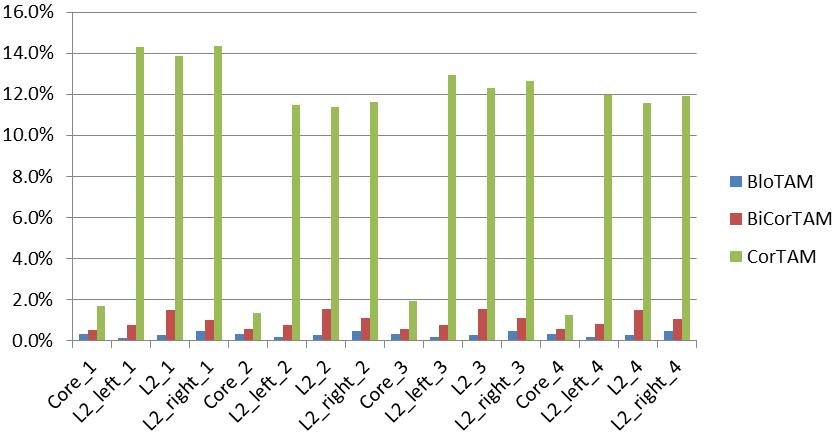
\includegraphics[width=1\textwidth,height=0.4\textheight]{EX1-PLK-ERROR}
  \caption{测例1各功能模块的静态功耗分析误差}
  \label{fig:ex1-plk-error}
\end{figure}
\begin{figure}[H]
  \centering
  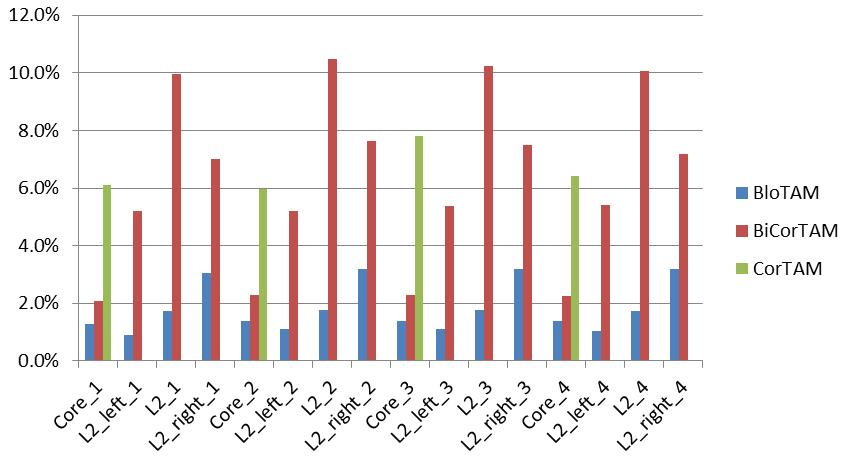
\includegraphics[width=1\textwidth,height=0.4\textheight]{EX1-TEMP-ERROR}
  \caption{测例1各功能模块温度的分析误差}
  \label{fig:ex1-temp-error}
\end{figure}


\section{本文方法计算速度的实验数据与分析}
\label{exp-speedup}
由于本文方法的算法复杂度非常低,本文采用16核的测例3(大测例)对其进行计算速度的验证。 在速度测试中,本文3种方法需要采用HotSpot软件对相关热阻的参数提取,由于芯片中有16个核、每核有4个模块, 所以本文方法需要进行64次HotSpot模拟,其耗时被称为建模时间$T_{Model}$,测试表明$T_{Model} = 3.447$ 秒(S)。当每种布图方案的相关热阻参数被提取出来后,本文方法基于这些参数、 采用式~\ref{equ:chap4:blotam-tii}、~\ref{equ:chap4:cortam-tpp}、式~\ref{equ:chap4:bicortam-tii} 对1000个输入向量进行温度与静态功耗计算,其耗时被称为热分析时间$T_{analysis}$; 建模时间与热分析时间之和被称为总耗时$T_{total}=T_{Model}+T_{analysis}$。 本文方法所提供的加速倍数$X$是HotSpot的耗时与本文方法耗时之比,其中不包含建模时间、 只采用热分析计算耗时进行加速比较的倍数被称为热分析加速倍数$X_{analysis}$, 而采用总耗时进行比较所得到的加速倍数被称为总耗时加速倍数$X_{total}$。
如表5所示,本文方法的总耗时主要消耗在建模时间上,只要提取出了模型参数,采用式~\ref{equ:chap4:blotam-tii}、 ~\ref{equ:chap4:cortam-tpp}、式~\ref{equ:chap4:bicortam-tii} 计算温度与静态功耗就是一个非常快速的计算过程,即$T_{analysis}$非常小, 只占$T_{total}$很小的部分。 与HotSpot软件相比,尽管本文3种方法分析计算的加速比$X_{analysis}$分别达到50、147、和66, 但由于$T_{analysis}$只占$T_{total}$很小的部分,所以本文3种方法总耗时的加速比只达到13、15、和14, 即本文3种方法的总耗时加速比近似相等,均可以获得满意的加速效果。

从表3-表5的算法精度与复杂度的比较结果可以看出:与HotSpot软件相比, 本文的BloTAM和BiCorTAM都可以在满足精度要求的前提下(热点温度误差小于2.2\%)获得满意的加速效果, 总耗时的加速比可以达到13倍和14倍。

\section{小结}
第~\ref{cha:SSTA}章介绍了采用自下而上的建模方法对MPSoC结构级热分析方法进行了探索, 提出了3种具有不同算法复杂度与精度的热分析方法: 模块级方法BloTAM、核级方法CorTAM、考虑本核内模块相互影响的改良核级方法BiCorTAM, 具有简单、高效、与现有简化模型兼容、易于扩展、能够解决温度对漏电流的影响等优点。 本章中大量的实验数据表明:对核数较多MPSoC进行热分析的时候,BloTAM和BiCorTAM均具有算法复杂度低和精度高的优点, 平均相对增量误差最大不超过3\%,同时可以获得14倍左右的运算加速效果,是一种较为理想的结构级热分析方法。










